\begin{refsection}
%-------------------------------------------------------------------------
%-------------------------------------------------------------------------
\chapter{Measuring optical imperfections in refractive lenses}\label{sec:measuring}
%-------------------------------------------------------------------------
%-------------------------------------------------------------------------

Surface metrology methods commonly applied to X-ray mirrors [\cite{Alcock2016, Vivo2019}] are not broadly employed for the metrology of X-ray lenses mainly due to their small apertures and steep parabolic surfaces (cf. Fig.~\ref{fig:ideal_CRL}) [\cite{Lyatun2015}]. Non-destructive methods using X-rays are often more appropriate for X-ray lens metrology. This section presents some of the commonly used at-wavelength metrology methods, with emphasis on X-ray speckle vectorial tracking (XSVT), the experimental technique used throughout this work. The metrology of single- and stacked 2D-Beryllium lens with $R=50~\mu$m is presented and the results are compared. A framework for calculating corrective optics for such stacked lenses is shown, along with the first correction prototypes and tests.

The experimental data shown in this chapter were taken on several beamtimes\footnote{Acknowledgements to Sébastien Bérujon and Ruxandra Cojocaru (BM05-ESRF); Xianbo Shi, Zhi Qiao, Michael Wojcik and Lahsen Assoufid (1-BM-APS); and to Carsten Detlefs (ID06-ESRF) for the help during the experimental sessions.} at the BM05 beamline - ESRF [\cite{Ziegler2004}] (from 2017 to 2018 - before the ESRF long shutdown for the EBS upgrade), at the 1-BM beamline - APS [\cite{Macrander2016}] (in 2019 during the ESRF long shutdown) and the ID06 beamline - ESRF [\cite{Kutsal_2019}] (in 2020 in the commissioning period of the ESRF-EBS upgrade).


%-------------------------------------------------------------------------
%-------------------------------------------------------------------------
\section{At wavelength-metrology}\label{sec:at_wavelength}
%-------------------------------------------------------------------------
%-------------------------------------------------------------------------

Surface metrology of X-ray optical elements is often done using visible spectral range [\cite{Alcock2016, Vivo2019}] even if, ultimately, they will be employed in a different spectral range. At-wavelength metrology is an umbrella term for measurements of optical elements at wavelengths closer to the ones they will be ultimately used - in the case of X-ray lenses, a few dozen kilo-electron-volts. What follows is a non-exhaustive description of commonly used techniques for quality control applied to X-ray lenses and their compliance to a parabolic shape. Other relevant at-wavelength characterisations of X-ray lenses such as X-ray small-angle scattering [\cite{Roth2014, Chubar2020}] or the impact of material micro-structures or shape errors on imaging [\cite{Chubar2020,Lyatun2020}] are not covered. 

The simplest techniques involve direct imaging the lens with X-rays by propagation-based phase-contrast imaging [\cite{Endrizzi2018}], since absorption contrast imaging has a very reduced contrast for a single lens. With such simple techniques, 2D shapes and distances can be measured (radiographs for controlling the distance and alignment between the parabolic surfaces of X-ray lenses). Still based on imaging techniques, X-ray laminography [\cite{Helfen2011,Roth2014}] and X-ray tomography [\cite{Landis2010,Narikovich2017}] of X-ray lenses provide a 3D reconstruction of the lens volume with high spatial resolution information. These techniques provide data on the shape of the refracting surfaces and the internal features (inhomogeneities) and can be used for modelling optical imperfections in refractive lenses. 


Another large family of experimental techniques used for lens metrology can be grouped under the wave-front sensing branch\footnote{With the advent of more coherent sources of X-rays as encapsulated by the emergence of $4^{\text{th}}$-generation synchrotrons and free-electron lasers, the topic of wavefront sensing has seen increased attention [\cite{Seaberg2019}].}. Wavefront-sensing is often employed as a beam-diagnostics tool for highly coherent sources [\cite{Seaberg2019}]. Two approaches are often used: \textit{i}-) the absolute wavefront after a specific optical element is measured and the global state of the wavefront is obtained or \textit{ii}-) a differential measurement is done with and without the optical element under investigation, the differences in the wavefront attributed to the addition of the optical element under test. Current wavefront-sensing techniques used for evaluating the phase errors of CRLs (or individual X-ray lenses) are: the Ronchi test, an interferometric technique that provides qualitative\footnote{It has been demonstrated that the Ronchi test can also retrieve quantitative information [\cite{Lee2010}], but it has not yet been applied to X-ray lenses metrology.} information on third-order optical aberrations [\cite{Nilsson2012, Uhlen2014}]; the use of X-ray Shack–Hartmann sensors [\cite{Mayo2004,Mikhaylov2020}]; the ptychographic reconstruction of the wavefront emerging from a strong focusing optics [\cite{Schropp2013,Sala2017,Seiboth2017}]; grating interferometry and all its variations [\cite{David2012,Koch2016,Grizolli2017}]; and the near-field-speckle-tracking-based methods [\cite{Berujon2013,Zdora2018,Berujon2020a}].

%-------------------------------------------------------------------------
%-------------------------------------------------------------------------
\subsection{X-ray (near field) speckle vector tracking (XSVT)}\label{sec:XSVT}%\addcontentsline{toc}{subsection}{-- X-ray (near field) speckle vector tracking (XSVT)}
%-------------------------------------------------------------------------
%-------------------------------------------------------------------------

The X-ray near-field-speckle-tracking is the chosen technique for systematic at-wavelength metrology of X-ray lenses at the ESRF\footnote{Other synchrotron facilities also offer X-ray lens metrology with the X-ray near field speckle imaging technique: 1-BM at the APS in the U.S.A. [\cite{Qiao2020}] and the B16 beamline at the Diamond Light Source in the U.K. [\cite{Sawhney2013}].} and is available at the BM05 beamline [\cite{Berujon2020a}] and most recently, at the ID06 beamline. The principal reasons for this choice are: \textit{i}-) the lower requirements on transverse- and longitudinal coherence [\cite{Zanette2014,Zdora2015,Wang2016}]; \textit{ii}-) no requirement of specially tailored optics (nor accompanying complicated alignment procedures) [\cite{Morgan2012,Wang2016}]; \textit{iii}-) successful benchmark against more established wave-front sensing techniques [\cite{Kashyap2016,Romell2017}]; and \textit{iv}-) its versatility as a metrology tool being able to measure mirrors, single- and stacked lenses [\cite{Berujon2020a}]. Although the basic principles of the several X-ray near-field-speckle-based techniques are the same, the focus is given to the X-ray (near field) speckle vector tracking (XSVT) as implemented and used for the metrology of single- and stacked X-ray lenses used in this work [\cite{Berujon2020a,Berujon2020}]. An interesting review of different techniques using X-ray near field speckle imaging is given by [\cite{Zdora2018a}] and [\cite{Berujon2020}].

%-------------------------------------------------------------------------
%-------------------------------------------------------------------------
\subsection{Foundation}\label{sec:foundation}
%-------------------------------------------------------------------------
%-------------------------------------------------------------------------

Near-field speckle is a manifestation in intensity of the summation of several complex electric fields when the amplitudes and phases of such fields have random values. The resulting intensities may be locally high due to constructive interference or low, due to destructive interference [\cite[\textit{\S1}]{Goodman2020}]. For a speckle pattern over a defined region of interest, the speckle contrast (or visibility) can be defined\footnote{Other definitions are commonly found in the literature: $v=\frac{I_\text{max}-I_\text{min}}{I_\text{max}-I_\text{min}}$ and $v=\frac{I_\text{max}-I_\text{min}}{2\overline{I}}$, where $I_\text{max}$ and $I_\text{min}$ are the maximum and minimum intensities found in the region of interest [\cite{Zdora2018a}].} as:
\begin{equation}\label{eq:visibility}
    v=\frac{\sigma_I}{\overline{I}},
\end{equation}
where $\sigma_I$ is the standard deviation and $\overline{I}$ is the mean value of the intensity value of the speckle pattern. In the X-ray regime, it appears when a sufficiently coherent X-ray beam is transmitted through matter with random spatial variation of $\delta$ and $\beta$, where the local optical path length varies significant when compared to the scale of the wavelength.

For a static random modulation of the wavefield (stationary diffuser\footnote{As opposed to time-varying modulation of the speckle-field as in [\cite{Morgan2010,Goikhman2015}].}), it has been demonstrated that the speckle-grains\footnote{Continous regions in space with a slowly-varying intensity that can be visually clustered together.} preserve shape and size for free-space propagation distances limited to:
\begin{equation}\label{eq:speckle_goodness}
z<\Delta_{\textbf{cl}_\perp}\xi k,
\end{equation}
where $\Delta_{\textbf{cl}_\perp}$ is transverse coherence length\footnote{cf. \textit{Spatial coherence} in \S\ref{sec:optical_coherence}~-~\textit{\nameref{sec:optical_coherence}}.} and $\xi$ is the typical transverse length of the modulator, that is, the region where the spatial variation of $\delta$ and $\beta$ is negligible [\cite{Cerbino2008}]. For propagation distances smaller than the imposed limit in Eq.~\ref{eq:speckle_goodness}, speckles can be used as a wavefront marker, since the transverse position of the speckle grains in two parallel planes along the propagation direction can be inferred geometrically. The near-field regime is of particular interest for the X-ray energy range, as very low wavelengths lead to an extended near-field regime. A speckle-pattern and the stationary diffuser used to generate it are shown in Fig.~\ref{fig:SpecklePattern}.

\begin{figure}[t]
        \centering
        {\includegraphics[width=0.6\linewidth]{figures/ch04/SpecklePattern.pdf}}
        \caption[Speckle-pattern and the stationary diffuser]{(a) Speckle-pattern measured at 17~keV at 800~mm downstream the with $\sigma_I=0.19$~a.u., $\overline{I}=0.99$~a.u. and $v\sim0.19$; (b) SEM image of the cellulose acetate membrane filters with mean pore size of 1.2~$\mu$m used as the stationary diffuser. The white bar in (b) represents 50~$\mu$m.} \label{fig:SpecklePattern}
\end{figure}

\begin{figure}[t]
        \centering
        {\includegraphics[width=1\linewidth]{figures/ch04/speckle_tracking.pdf}}
        \caption[Tracking of speckle grain]{Tracking of speckle grains. The highlighted grains in yellow and red are inside the sample and have their transverse position changed. The highlighted grain in blue is outside the lens active area and has no apparent shift in the transverse position. The speckle grains in the image of the sample have their intensity reduced due to absorption of the bulk material. The sample is a single 2D-Beryllium lens with nominal radius $R=50~\mu\text{m}$, geometric aperture $A_{\diameter}\sim440~\mu\text{m}$. The data was collected $\sim$800mm downstream the speckle-membrane at 17~keV.} \label{fig:speckle_tracking}
\end{figure}

\begin{figure}[t]
        \centering
        {\includegraphics[width=0.6\linewidth]{figures/ch04/speckle_tracking2.png}}
        \caption[Speckle-based imaging geometry]{Generic speckle-based imaging measurement geometry for the XSVT technique and the origin of the displacement vector $\nu$. From left to right: X-ray beam, speckle-membrane, sample and 2D imaging detector. The distance between sample and detector is given by $d$, the deflection angle is $\alpha$ and the transverse displacement vector in the detector plane is $\nu$.} \label{fig:speckle_tracking2}
\end{figure}

Based on the uniqueness of each speckle grain, speckle-imaging-based techniques rely on identifying similar patterns in two different images sets: reference image and image in the presence of the probe (perturbed) - cf. Fig.~\ref{fig:speckle_tracking}. The computer implementations used for numerically tracking the lateral displacement of the speckle grains in the detector plane vary: cross-correlation peak calculation [\cite{Berujon2012, Morgan2012}] and the least-square-minimisation [\cite{Zanette2014, Zdora2017}] are the two most used methods\footnote{Recently, a Euclidean-distance minimisation of the wavelet-transform method has been reported. Compared to correlation-based techniques it is less computationally demanding and more robust to noise [\cite{Qiao2020b}].}$^{,}$\footnote{Regardless of the tracking method, the displacement vector $\nu$ should be equivalent, as it is intimately linked to the sample shape and material.}. The lateral displacement of the speckle grain in the detector plane between the reference and the disturbed image is given by the displacement vector $\nu=(\Delta_x,\Delta_y)$, where $\Delta_x$ and $\Delta_y$ are the respective horizontal and vertical displacements of the speckle grain in the presence of the sample - cf. Fig.~\ref{fig:speckle_tracking2}. With knowledge of the distance between sample and detector $d$, it is possible to reconstruct the deflection angle $\alpha=(\alpha_x,\alpha_y)\approx\nu/d$. The deflection angle, the wave-field phase $\phi(x,y)$ and wavefront $\mathcal{W}(x,y)$ are related by:
\begin{equation}\label{eq:wavefront_gradient}
    k\frac{\nu}{d} \approx k \alpha = \nabla\phi(x,y) = k \nabla\mathcal{W}(x,y).
\end{equation}
The beam phase $\phi(x,y)$ or wavefront $\mathcal{W}(x,y)$ can be retrieved by numerical integration of the phase gradients obtained experimentally.

%-------------------------------------------------------------------------
%-------------------------------------------------------------------------
\subsection{Experimental setup}\label{sec:experimental_setup}
%-------------------------------------------------------------------------
%-------------------------------------------------------------------------

\begin{figure}[t]
        \centering
        {\includegraphics[width=0.7\linewidth]{figures/ch04/BM05.pdf}}
        \caption[Speckle-based imaging experimental setup at the BM05 beamline, ESRF.]{Generic speckle-based imaging experimental setup as originally implemented in the BM05 beamline at the ESRF. \textbf{right to left}: an X-ray source (bending magnet) delivers a beam that is  monochromatised by Si(111) double crystal monochromator down to a bandwidth of $\Delta \text{E}/\text{E}\approx10^{-4}$. The now monochromatised beam hits the speckle-generator at a distance $R_S$ from the source. The stationary diffuser is composed of several piled up cellulose acetate membrane filters with a mean pore size of 1.2~$\mu$m. The membranes are mounted on a (piezoelectric) nano-positioner transverse translation stage, so that the membranes can be scanned on the $xy-$plane. At a distance $l$ downstream the membrane, the sample is placed and aligned as to the optical axis. Further downstream the probe, at a distance $d$, a 10~$\mu$m thick LSO:Tb scintillator converts the X-rays into visible light. The scintillator is imaged into a CMOS PCO Edge 4.2 or a FReLoN camera (2048 $\times$ 2048 pixels), which is coupled with a 10$\times$ magnification microscope objective to reach as the theoretical pixel size of about $\sim0.62\times0.62~\mu$m$^2$. Such experimental setup, without any structural change, was later on used at the 1-BM (APS) and ID06 (ESRF) beamlines. The X-ray source at the ID06 is an undulator and not a bending magnet as depicted here.} \label{fig:BM05}
\end{figure}

\begin{figure}[t]
        \centering
        {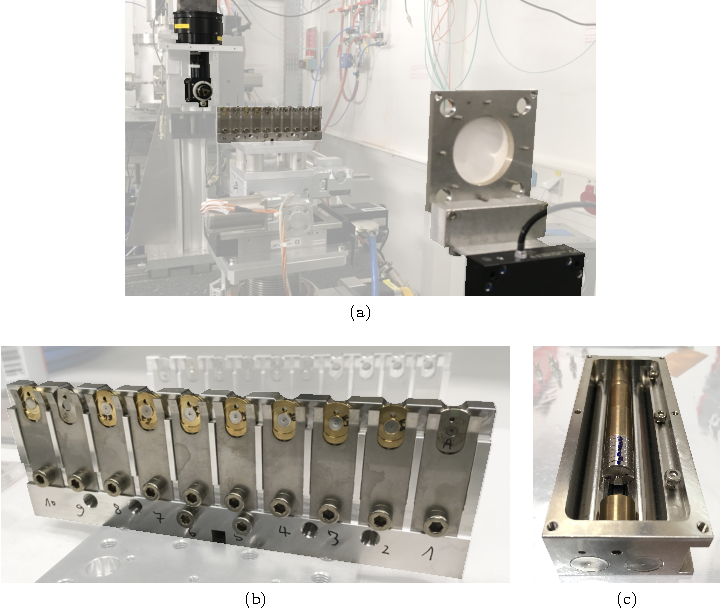
\includegraphics[width=.7\linewidth]{figures/ch04/experimental_setup.pdf}}
        \caption[Experimental setup at the BM05 beamline, ESRF.]{(a) image inside the experimental hutch of the BM05. The picture highlights the three main components shown schematically in Fig.~\ref{fig:speckle_tracking2}: the detector in the back-plane, the sample-holder specially designed to hold up to 10 lenslets for batch measurements and the speckle-membrane mounted in a (piezoelectric) nano-positioner in the first plane. (b) typical lenslets mounted on the holder designed to provide easy alignment of the lenses in the X-ray beam and ensure repeatable positioning in the lens mount. This holder is designed for single-lens measurement. (c) stacked lenses require a different mounting for metrology.} \label{fig:experimental_setup}
\end{figure}


X-ray speckle imaging (SBI) can be implemented in several geometries depending on the metrology subject (mirrors, strong focusing mirrors, lenses, stacked lenses) and mode (absolute or differential) - cf. [\cite{Berujon2020a}]. In this section the X-ray (near field) speckle vector tracking (XSVT), a differential metrology mode, as originally implemented at BM05 and shown in Figs.~\ref{fig:speckle_tracking2}, \ref{fig:BM05} and \ref{fig:experimental_setup} is described.

\subsubsection*{Illumination}

Unlike other wavefront sensing techniques, speckle-based metrology has low requirements on transverse and longitudinal coherence\footnote{Phase-contrast with low-coherence sources has, in fact, been demonstrated [\cite{Cloetens1996, Wilkins1996, Pfeiffer2006, Munro2012}].} as demonstrated by [\cite{Zanette2014,Zdora2015,Wang2016}]. The degree of lateral coherence of the illumination is intimately connected with two important factors: the speckle contrast (cf. Eq.~\ref{eq:visibility}) and the propagation distance where shape and size of the speckle grains are preserved (cf. Eq.~\ref{eq:speckle_goodness}). X-rays with lower transverse coherence will produce speckles with low visibility (smeared out or blurred image \todo{- cf. Fig.~\ref{fig:coherence_vs_visibility}}) and the numerical process of tracking signals will lose some of its accuracy. For metrological applications, a minimum contrast of 0.1 (Eq.~\ref{eq:visibility}) is expected [\cite{Berujon2020a}]. A reduced propagation distance $d$ between the sample and the detector (cf. Fig.~\ref{fig:speckle_tracking2} and \ref{fig:BM05}) arising from a reduced coherence length $\Delta_{\textbf{cl}_\perp}$ (Eq.~\ref{eq:speckle_goodness}) diminishes the angular sensitivity and will impact on the residual height error measurement sensitivity. When selecting an X-ray source, a higher degree of transverse coherence is preferred. Nonetheless, bending magnets\footnote{At BM05, a bending magnet was the X-ray source until the ESRF-EBS upgrade long shutdown (December 2018). The BM was decommissioned in favour of a much shorter and brighter 2-pole wiggler, installed early 2020. All the data collected at BM05 was taken before this upgrade.} are often used at beamlines where speckle-imaging-based metrology is available\footnote{As of the writing of this thesis, the beamlines the routinely offer X-ray lenses metrology with speckle-based-imaging are the BM05 (ESRF) [\cite{Berujon2020a}], 1-BM (APS) [\cite{Qiao2020}] and B16 (DLS) [\cite{Sawhney2013}].}. 

Choosing the experiment energy\footnote{ The energy chosen for all metrology experiments is $\text{E}=17~$keV with $\Delta \text{E}/\text{E}\approx10^{-4}$ by using a Si(111) DCM. This energy was originally set at the BM05, as early experiments took place there, but was later adopted at experiments in other beamlines to facilitate direct comparison at all stages of the data-analysis.} for X-ray lens metrology is reaching a compromise between several competing constraints. For a fixed distance $d$, the energy should be high enough so that the speckle grains being transmitted through the lens geometric aperture are not excessively deformed by focusing at the detection plane - the higher the energy, the longer the focal length of a X-ray lens is (cf. Eq.~\ref{eq:CRL_classic}). Excessive deformation of the transmitted speckle field causes the tracking to fail in delivering credible results. Higher energy is also beneficial when considering the limit to the distance $d$ imposed by Eq.~\ref{eq:speckle_goodness}. On the other hand, increasing the energy decreases the coherent fraction of the emitted beam, which in turn reduces the speckle visibility\footnote{Slitting down the beam and increasing the propagation distance from source to speckle-membrane ($R_s$ in Fig.~\ref{fig:BM05}) help to increase the coherence length at the expense of photon flux - cf. van-Cittert-Zernike theorem in [\cite[\textit{§4.4.4}]{Mandel1995}] or the applicability to SR in [\cite[\textit{§4}]{Geloni2008}].}. Lastly, the source spectrum (Fig.~\ref{fig:emission}) has also to be considered, as a higher photon flux allows for shorter acquisition time, meaning that experiments require less time and possible instabilities (vibrations, long time drifts and other external perturbations) have a lower impact on the acquired data. Requirements on the illumination monochromaticity are not stringent for SBI, but metrology of X-ray lenses require narrow bandwidths as they suffer from intrinsic chromatic aberrations. In order to secure a good lateral resolution, a Si(111) double crystal monochromator (DCM)\footnote{An experimental comparison between the metrology data obtained with a Si(111) DCM with $\Delta \text{E}/\text{E}\approx10^{-4}$ and a multi-layer monochromator with $\Delta \text{E}/\text{E}\approx10^{-2}$ shows very good agreement between both data-sets [\cite[\textit{\S3.3.3}]{Berujon2020a}].} is usually used to bring down the bandwidth to $\Delta \text{E}/\text{E}\approx10^{-4}$.

\subsubsection*{Speckle membrane}

Unlike other wavefront techniques that require specially tailored optics that may need laborious alignment procedures such as reference phase-objects (Siemens star) or gratings, SBI requires a transmission element with transversely distributed random optical path differences capable of producing speckle-grains that covers a few pixels (<10 pixels) at the detector with visibility of $ v>0.1$ [\cite[\textit{\S2.3}]{Berujon2020a}]. Early experiments were done by stacking commercially available abrasive paper (sandpaper) until the desired speckle pattern was obtained\footnote{More recently guidelines helping to choose the appropriate sandpaper grain size (grit) for an experimental setup were published by [\cite{Tian2020}].} [\cite{Morgan2012, Wang2016}]. The choice of modulator depends on the experiment energy and the detector, but generally, static granular materials, sandpaper of diverse grits and filters with micrometric pore-sizes are used\footnote{Experiments shown here used a stack of cellulose acetate membrane filters with a mean pore size of 1.2~$\mu$m used as the stationary diffuser.}. Low transmission, poor time stability and/or the presence of strong diffraction are characteristics that should be avoided when choosing a speckle generator. Due to the random nature of the wavefront (static) modulation, the membrane does not require alignment concerning the beam. 

XSVT is a a scanning technique and customary\footnote{More details in data acquisition are provided by \S\ref{sec:data}~-~\textit{\nameref{sec:data}}.} $N$ reference images are taken at $N$ different transverse positions of the speckle generator in respect to the optical axis. The probe is put into the beam and another set of $N$ images at the exact previous $N$ positions are taken - cf. orange arrows in Fig.~\ref{fig:speckle_tracking2}. The reproducibility of the $N$ transverse positions is of key importance as the difference in the speckle grain positions from reference to sample image is attributed to the probe modulation of the beam. To ensure that for any $j^\text{th}~(j\in[1,2,...,N])$ pair of images the position of the speckle generator is as close as a fraction of effective pixel size, the modulator is mounted in a (piezoelectric) nano-positioner with a travel range of at least a millimetre. 

\subsubsection*{Sample}

X-ray speckle vectorial tracking is a very attractive technique as it can measure weak-focusing optics as well as very strong focusing systems - cf. [\cite{Berujon2020a}] for some examples. Typically, two types of optical elements are routinely measured at the ESRF: individual lenses and moderately focusing CRLs. Fig.~\ref{fig:experimental_setup}(b) and (c) shows typical probes in their holder. Single lenses are mounted in an in-house-designed holder conceived to hold up to 10 lenslets, allowing serial measurements and minimising manual intervention to change samples. Stacked lenses are measured on typical casings. The lens holder has to be mounted in a support that can move transversely to the beam ($xy-$plane) and has yaw, pitch, and roll rotations\footnote{Yaw is a rotation around the $z-$axis, the pitch is around the $y-$axis and roll, the $x-$axis.} to compensate for the residual phase errors introduced by misalignments - cf. \S\ref{sec:misalignments}~-~\textit{\nameref{sec:misalignments}}. 

\subsubsection*{Detection}

Although subpixel resolution for XSVT has been recently reported [\cite{Qiao2020b}], generally, the lateral resolution of the 2D surface maps obtained with XSVT is limited to the detector effective pixel size, hence 2D high-resolution imaging detectors are used for speckle-based imaging. In real-space imaging with X-rays, it is common to use indirect detection. Converting X-rays into visible-light and subsequently imaging it into a pixelated detector allows profiting from very small pixel sizes typical of sensors designed for visible-light.

A typical detection system\footnote{The detection systems use at the ESRF are composed of a 10~$\mu$m thick LSO:Tb scintillator that is imaged into an sCMOS PCO Edge 4.2 or a FReLoN CCD camera (2048 $\times$ 2048 pixels), which is coupled with a 10$\times$ magnification microscope objective to reach a theoretical pixel size of about $\sim0.62\times0.62~\mu$m$^2$. At the APS, the scintillator used is a 100~$\mu$m thick LuAG:Ce imaged into an Andor Neo sCMOS camera with 2560 $\times$ 2180 pixels also with a 10$\times$ magnification resulting in a pixel size of $\sim0.65\times0.65~\mu$m$^2$.} is composed of three main parts: \textit{i}-) the scintillator, which is responsible for converting the X-rays into visible light. Its choice is a compromise between the yield in converting X-ray photons in visible photons and image sharpness: a thin scintillator will generally result in a sharper image, but at a cost of a reduced photon flux, while a thicker one will generate more light, but due to scattering in the bulk material, a less sharp image will be available; \textit{ii}-) the transport optics that magnifies and images the scintillator in the sensor plane, but also may introduce aberrations to the system, but can be calibrated with the XSVT technique - cf. [\cite[\textit{\S2.2}]{Berujon2020a}]; and \textit{iii}-) the imaging sensor, which ideally should be a low-noise 2D pixelated sensor with fast read-out. The final effective pixel size is a convolution of the contributions from the choice of scintillator, magnification and point spread function of the transport optics and the imaging device.

\begin{figure}[t]
        \centering
        {\includegraphics[width=.7\linewidth]{figures/ch04/speckle_data.pdf}}
        \caption[X-ray (near field) speckle vector tracking (XSVT)]{X-ray (near field) speckle vector tracking (XSVT). In the differential mode, two data-sets are taken: the reference and the one with the probe. Each of the $j^\text{th}$ from a particular data-set is taken at a different transverse scan position of the speckle-generator across the X-ray beam, however, for a particular $j^\text{th}$ image-pair
        (reference and probe) the exact same diffuser position is maintained. A reference intensity vector $I_{\text{reference}}(x_l,y_m,j)$ (green) is searched in the probe stack, ROI centred around $(x_l,y_m,j)$, where $I_{\text{probe}}(x_{l+\Delta l},y_{m+\Delta m},j)$ vectors are calculated. The purple signal is a well matched signal, while the yellow signal shows the neighbouring-pixel intensity vector $I_{\text{probe}}(x_{l-2},y_{m-2},j)$.}\label{fig:data_tracking}
\end{figure}


%-------------------------------------------------------------------------
%-------------------------------------------------------------------------
\subsection{Data acquisition, processing and analysis}\label{sec:data}
%-------------------------------------------------------------------------
%-------------------------------------------------------------------------

\subsubsection*{Data acquisition}

Early implementations of X-ray speckle-tracking for metrology consisted in acquiring two images: the reference- and the probe-image with the same speckle pattern (cf. Fig.~\ref{fig:speckle_tracking}). The algorithms used to match the patterns in both images rely in setting in the reference image a small window around a pixel of interest, that is, $w_\text{reference}(x_l,y_m)$ and searching for this (possibly distorted) pattern it in a larger window in the sample image: $w_\text{probe}(x_l,y_m)$. The reference window is rastered through the whole sample image ($L\times M$ pixels), to reconstruct two 2D displacement maps (horizontal and vertical) with lateral resolution limited to the speckle-grain size. In order overcome the low spatial resolution from XST, XSVT relies on transversely scanning\footnote{The nature of the scan is not particularly relevant for the data analysis in this particular metrology mode. A random set on $N$ points distributed in the $xy-$plane can be used, provided repeatability in positioning the speckle generator is a fraction of the effective detector pixel size.} the speckle-generator across the X-ray beam and taking images at the $N$ different points of the scan. Once the reference data-set is taken, the probe is inserted in the beam and the scan is repeated at the exact same diffuser position. Each data set (reference and probe) contains $N_{L\times M}$ images where the $j^\text{th}~(j\in[1,2,...,N])$ image in each stack indicates the same transverse coordinates of the scatterer scan - cf. Fig.~\ref{fig:data_tracking}. For a sufficiently large $N$, a locally uncorrelated intensity vector can be obtained by sampling each $j^\text{th}$ image of the reference data-set around a pixel coordinate $(x_l,y_m)$ with $l\in[1,2,...,L]$ and $m\in[1,2,...,M]$. This reference signal $I_{\text{reference}}(x_l,y_m,j)$ is shown in green in Fig.~\ref{fig:data_tracking}. A ROI centred in $(x_l,y_m)$ is set on the probe data-set and for each pixel coordinate within this ROI, that is $(x_{l+\Delta l},y_{m+\Delta m})$, a corresponding intensity vector is also obtained: $I_{\text{probe}}(x_{l+\Delta l},y_{m+\Delta m},j)$ - cf. magenta and orange signals in Fig.~\ref{fig:data_tracking}. The 1D $I_{\text{reference}}(x_l,y_m,j)$ vector is compared\footnote{Cross-correlation peak calculation [\cite{Berujon2012, Morgan2012}], least-square-minimisation [\cite{Zanette2014, Zdora2017}] or Euclidean-distance minimisation of the wavelet-transform of the reference- and probe- vectors [\cite{Qiao2020b}].} individually to each of the $I_{\text{probe}}(x_{l+\Delta l},y_{m+\Delta m},j)$ vectors - in this work the cross-correlation peak calculation is the preferred method for speckle-vector tracking [\cite{Berujon2012, Morgan2012}]; Fig.~\ref{fig:cross-correlation-map} shows the normalised cross-correlation values for a particular probe, which is used to evaluate the convergence of the method. By repeating this procedure for all $L\times M$ pixels, it is possible to obtain two 2D displacement maps (vertical and horizontal) with lateral resolution down to $\sim$~effective-pixel-size of the detector at the expense of increased data-collection and data-processing [\cite{Berujon2016,Berujon2020}].

\begin{figure}[t]
        \centering
        {\includegraphics[width=.5\linewidth]{figures/ch04b/radio_corr_map.pdf}}
        \caption[Normalised cross-correlation map]{(a) radiography of a 2D-Beryllium lens with $R=50~\mu$m measured at 17~keV with $d=800$~mm and pixel size $\Delta_\text{pixel}= 0.63~\mu$m. The different penetration depths of the parabolic profiles cause the reduction of the geometric aperture, evidenced by the two concentric rings. (b) the normalised cross-correlation peak for the vector tracking algorithm. Regions with darker colours have lower peaks.}\label{fig:cross-correlation-map}
\end{figure}

\begin{figure}[t]
        \centering
        {\includegraphics[width=.6\linewidth]{figures/ch04b/gradients.pdf}}
        \caption[Recovered phase gradient and residues]{(a) horizontal and (c) vertical gradients phase gradients for the 2D-Beryllium lens with $R=50~\mu$m measured at 17~keV with $d=800$~mm and pixel size $\Delta_\text{pixel}= 0.63~\mu$m - cf. Fig.~\ref{fig:cross-correlation-map}.}\label{fig:gradients}
\end{figure}

\begin{figure}[t]
        \centering
        {\includegraphics[width=1\linewidth]{figures/ch04b/recovered_thickness.pdf}}
        \caption[Recovered figure errors in projection approximation]{(a) Recovered figure errors in projection approximation of a 2D-Beryllium lens with $R=50~\mu$m measured at 17~keV with $d=800$~mm and pixel size $\Delta_\text{pixel}= 0.63~\mu$m, (b) Zernike circle polynomial fit of the figure errors and (c) the residues from the fit. The coefficients of the fit are shown in (d). (e) Power spectrum density of the horizontal and vertical cuts around the centre of lens.}\label{fig:recovered_thickness}
\end{figure}

\subsubsection*{Data processing \& analysis}

The phase gradients $\nabla\phi(x,y)$ can be obtained from the two displacement maps by multiplying them by the wavenumber $k$ and dividing the product by the distance between the sample and detector ($d$) - cf. Eq.~\ref{eq:wavefront_gradient}. An example of the horizontal and vertical gradient for a 2D-Beryllium lens with $R=50~\mu$m measured at 17~keV with $d=800$~mm and pixel size $\Delta_\text{pixel}= 0.63~\mu$m is shown in Fig.~\ref{fig:gradients}(a)-(b), where the mismatch between front- and back- focusing surfaces is evident - cf. Fig.~\ref{fig:cross-correlation-map}. Ideal lenses have phase gradients with linear dependency on the focusing direction\footnote{From Eq.~\ref{eq:aux_funcs_transb} and Eq.~\ref{eq:ProjecThick}: 
\begin{align*}
    \nabla\phi(x,y) & = \Bigg(\frac{\partial \phi(x,y)}{\partial x},\frac{\partial \phi(x,y)}{\partial y}  \Bigg) = -2k\delta\Bigg(\frac{x}{R_x},\frac{y}{R_y}\Bigg),
\end{align*}{}
which is a linear function.} and slope of the linear phase-gradient in the focusing direction is inversely proportional to the radius of curvature of the X-ray lens, which can be retrieved with the knowledge of the experiment energy and lens material (refraction index decrements). It is possible to access the phase gradient residues (or errors) by removing a linear fit from the gradients, which is shown in Fig.~\ref{fig:gradients}(c)-(d). In order to recover the thickness profile in projection approximation from the phase gradient (or from the residual phase gradient), the first necessary step is the numerical integration\footnote{More on numerical integration of gradient fields in [\cite{Huang2015}] and [\cite{Agrawal2006}].} of the differential fields, which is done using either the Frankot-Chelappa method [\cite{Frankot1988}] or the Harker-O'Leary method ($\text{grad2surf}$) [\cite{Harker2015}]. The profile resulting from the 2D integration of the (residual) phase gradients can be converted into thickness in projection approximation by (cf. Eq.~\ref{eq:aux_funcs_transb}):
\begin{align}\label{eq:recovered_thickness}
     \Delta_z(x,y)&=-\frac{\phi(x,y)}{k\delta}.
\end{align}{}
Eq.~\ref{eq:recovered_thickness} is based on the assumption that the X-ray lens is has a refraction index decrement $\delta$ with no variations in $(x,y,z)$. Eq.~\ref{eq:recovered_thickness} also justifies the use of a monochromator in the experimental setup (cf. Fig.~\ref{fig:BM05}), since $\delta$ has an important energy dependency.

The figure errors from a lens can be obtained by: \textit{i}-) integrating the phase gradients, fit and removal of either a cylinder with parabolic section or a paraboloid of revolution depending on whether the lens is a 1D or 2D focusing element. The treatment shown in Eq.~\ref{eq:recovered_thickness} is applied to this residual phase; or by \textit{ii}-)direct integration of the residual phase gradients and application of Eq.~\ref{eq:recovered_thickness} to the integrated field. The residual thickness in projection approximation is shown in Fig.~\ref{fig:recovered_thickness}(a). Valuable metrological information such as the RMS value of the figure errors; the decomposition of the wavefront into orthonormal polynomials (cf. \S\ref{sec:orthonormal_polynomials}~-~\textit{\nameref{sec:orthonormal_polynomials}}) for the systematic study of the optical imperfections; and the power spectral density (PSD) of horizontal- and vertical- profile cuts showing the spatial frequency distribution of the optical errors can all be obtained from the residual thickness profile as shown in Fig.~\ref{fig:recovered_thickness}. The recovered thickness profile in Fig.~\ref{fig:recovered_thickness}(a) can be directly used as a $\Delta_z(x,y)$ map in Eq.~\ref{eq:transmission_operator} to simulate the effects of optical imperfections in X-ray lenses as discussed in \S\ref{sec:metrology_data}~-~\textit{\nameref{sec:metrology_data}} from \S\ref{sec:other_sources}~-~\textit{\nameref{sec:other_sources}}. 


\subsubsection*{Measurement sensitivity}

Finally, some considerations on the measurement sensitivity. Considering an ideal detection system with effective pixel size $\Delta_\text{pixel}$, the minimum measurable deflection angle is:
\begin{align}\label{eq:alpha_min}
    \alpha_\text{min}=\eta\frac{\Delta_\text{pixel}}{d},
\end{align}
where $\eta$ is a correction factor for the pixel size\footnote{A factor $\eta<1$ implies subpixel accuracy, while $\eta>1$
means image resolution deterioration.}. Consider that the probe can be laterally sampled with the detector spatial resolution $\eta\Delta_\text{pixel}$ as shown in Fig.~\ref{fig:sensitivity}(a). Each projected pixel will have a mean height value and the minimum detectable height difference between two adjacent pixels is $\Delta{z_{min}}$. The angle $\alpha_\text{min}$ can be attributed to refraction caused by the local slope $\vartheta$ between two adjacent projected pixel - cf. Fig.~\ref{fig:sensitivity}(b). A ray that is parallel to the optical axis will intercept this local slope at an angle $\theta_1=\vartheta$ and will be refracted with an angle $\theta_2=\vartheta+\alpha_\text{min}$. With the law of refraction (Eq.~\ref{eq:refraction}) it is possible to estimate\footnote{From Fig.~\ref{eq:XSVT_resolution}(a) one obtains: $\tan(\vartheta)=\cfrac{\Delta{z_{min}}}{\eta\Delta_\text{pixel}}$. Using $n_1=1$, $n_2=1-\delta$, $\theta_1=\vartheta$ and  $\theta_2=\vartheta+\alpha_\text{min}$ in the law of refraction (Eq.~\ref{eq:refraction}): $\sin(\vartheta)=(1-\delta)\sin(\vartheta+\alpha_\text{min})$. Writing $\sin(\vartheta+\alpha_\text{min})=\sin(\vartheta)\cos(\alpha_\text{min})+\sin(\alpha_\text{min})\cos(\vartheta)$ and collecting terms, one obtains Eq.~\ref{eq:XSVT_resolution}.
% \begin{align*}
%     1\cdot\sin(\vartheta)&=(1-\delta)\sin(\vartheta+\alpha_\text{min})\\
%     &=(1-\delta)[\sin(\vartheta)\cos(\alpha_\text{min})+\sin(\alpha_\text{min})\cos(\vartheta)]\\
%     &=\frac{\sin(\alpha_\text{min})\cos(\vartheta)(1-\delta)}{1-(1-\delta)\cos(\alpha_\text{min})}.
% \end{align*}
% Rearranging terms:
% \begin{align*}
%     \tan(\vartheta)=\frac{\Delta{z_{min}}}{\eta\Delta_\text{pixel}}=\frac{\sin(\vartheta)}{\cos(\vartheta)}=\frac{\sin(\alpha_\text{min})}{\cfrac{1}{1-\delta}-\cos(\alpha_\text{min})}.
% \end{align*}
} the longitudinal sensitivity of the XSVT as: 
\begin{align}\label{eq:XSVT_resolution}
\Delta{z_{min}}=\eta\Delta_\text{pixel}\cdot\frac{\sin(\alpha_\text{min})}{\cfrac{1}{1-\delta}-\cos(\alpha_\text{min})}.
\end{align}
From Eq.~\ref{eq:XSVT_resolution}, it clear that longitudinal resolution of the XSVT technique depends on several factors: distance between speckle-generator and detector $d$; material and experiment energy expressed as index of refraction decrement $\delta$; and the the effective pixel size $\Delta_\text{pixel}$, which is directly impacted by the PSF of the transport optics of the imaging system. Other factors that contribute to the reduction in lateral resolution (increase $\eta$): \textit{i}-) the thickness of the scintillator used (blurring from thicker materials), \textit{ii}-) temporal beam-instabilities as they may reduce the apparent transverse coherence if the integration time of the detector is longer than the instabilities period; \textit{iii}-) vibrations of the sample holder with amplitudes larger than half of the pixel size and faster than the acquisition time. A low reproducibility of the speckle-generator membrane positioning in the X-ray beam and decreases the sensitivity as any change in speckle position in a differential measurement, regardless of its origin, is attributed to the sample modulation of the wavefront markers. Fig.~\ref{fig:sensitivity_2} shows the XSVT longitudinal sensitivity ($\Delta{z_{min}}$) for three common used materials for refractive optics manufacturing. 

\begin{figure}[t]
        \centering
        {\includegraphics[width=0.5\linewidth]{figures/ch04b/sensitivity.pdf}}
        \caption[XSVT sensitivity calculation sketch]{Sketch for aiding the calculation of the XSVT longitudinal sensitivity. The lateral resolution to which the probe is sampled generates a local slope between adjacent pixels (red dashed line with inclination given by $\vartheta$). A beam parallel to the optical axis (purple) hits the sample is refracted with an angle $\theta_2$.}\label{fig:sensitivity}
\end{figure}

\begin{figure}[t]
        \centering
        {\includegraphics[width=1.0\linewidth]{figures/ch04b/sensitivity_2.pdf}}
        \caption[XSVT sensitivity calculation]{X-ray speckle vectorial tracking longitudinal sensitivity ($\Delta{z_{min}}$) for three common used materials for refractive optics manufacturing. The solid red line indicates the performance of the method at 10~keV, while the solid green line for 30~keV. The dashed purple line indicates the experimental performance at 17~keV (used energy for such experiments in this work.). Black point-dashed line indicates the nominal pixel size of the imaging detector $\Delta_\text{pixel}=0.65~\mu$m. Curves calculated using Eq.~\ref{eq:XSVT_resolution}.}\label{fig:sensitivity_2}
\end{figure}

\newpage
\newpage

%-------------------------------------------------------------------------
%-------------------------------------------------------------------------
\section{Single lens measurements}
%-------------------------------------------------------------------------
%-------------------------------------------------------------------------

%-------------------------------------------------------------------------
%-------------------------------------------------------------------------
\section{Stacked lenses measurements}
%-------------------------------------------------------------------------
%-------------------------------------------------------------------------

%-------------------------------------------------------------------------
%-------------------------------------------------------------------------
\section{Corrective optics}
%-------------------------------------------------------------------------
%-------------------------------------------------------------------------
\subsection{Design}\label{sec:design}

\subsection{Prototype}\label{sec:prototype}

\subsection{Expected performance}\label{sec:performance}

\subsection{Early tests}\label{sec:prototype_testing}

% %-------------------------------------------------------------------------

$\blacksquare$
\addcontentsline{toc}{section}{References}
\printbibliography[heading=subbibliography]
\end{refsection}

